%=================================================================
% Two Streams, Four Architectures — MDPI MTI submission
% SHORT VERSION, target <= 17 pages INCLUDING references.
%
% Built from main.tex. Differences, all length-driven:
%   * Introduction paragraphs 1-2 are the author's own hand-written text, kept
%     verbatim apart from two typo fixes; the scenario figure is added back.
%   * Every figure caption is three lines or fewer.
%   * Methods no longer restates the leakage counts that Results reports.
%   * The capacity-convention argument is stated once, in Experimental Settings,
%     instead of twice.
%   * Detector-in-the-loop and qualitative behaviour are one subsection.
%   * Floats use [htbp] rather than [H] so pages pack.
% No result, no limitation and no citation was removed. main.tex is unchanged.
% Compile: tectonic main_short.tex   (or pdflatex + bibtex on Overleaf)
%=================================================================
\documentclass[mti,article,submit,moreauthors]{Definitions/mdpi}

%=================================================================
% MDPI internal commands - do not modify
\firstpage{1}
\makeatletter
\setcounter{page}{\@firstpage}
\makeatother
\pubvolume{1}
\issuenum{1}
\articlenumber{0}
\pubyear{2026}
\copyrightyear{2026}
\datereceived{ }
\daterevised{ }
\dateaccepted{ }
\datepublished{ }
\externalbibliography{yes}

% Float placement. LaTeX's defaults reserve so much of each page for text that a
% page carrying two large floats is left half empty; across seven figures and four
% tables that costs several pages of white space. These are the standard
% relaxations: they change only where floats are allowed to sit, never the
% typography, the content, or the class file.
\renewcommand{\topfraction}{0.92}
\renewcommand{\bottomfraction}{0.85}
\renewcommand{\textfraction}{0.06}
\renewcommand{\floatpagefraction}{0.80}
\setcounter{topnumber}{3}
\setcounter{bottomnumber}{2}
\setcounter{totalnumber}{4}

%=================================================================
% Full title of the paper (Capitalized)
\Title{Two Streams, Four Architectures: A Leakage-Free, Statistically Rigorous Benchmark for Pedestrian Crossing-Intention Prediction on PIE}

% Author Orchid ID: enter ID or remove command
\newcommand{\orcidauthorA}{0000-0000-0000-0000} % PLACEHOLDER

% Authors, for the paper (add full first names)
\Author{PLACEHOLDER Firstname Lastname $^{1,}$*\orcidA{} and PLACEHOLDER Firstname Lastname $^{1}$}

% MDPI internal command: Authors, for metadata in PDF
\AuthorNames{PLACEHOLDER Firstname Lastname, PLACEHOLDER Firstname Lastname}

% Affiliations / Addresses
\address{%
$^{1}$ \quad PLACEHOLDER Department, PLACEHOLDER University, PLACEHOLDER City, PLACEHOLDER Country; placeholder@example.com}

% Contact information of the corresponding author
\corres{Correspondence: placeholder@example.com}

% Abstract — 197 words
\abstract{Predicting whether a pedestrian is about to cross is a core requirement for automated vehicles, and the PIE dataset is its standard testbed. We first show that the observation windows commonly extracted from PIE contain the event they are meant to precede: measured against the dataset's own per-frame crossing annotation, 67.9\% of crossing sequences are observed while the pedestrian is already crossing. Re-anchoring every window at the labelled crossing event, with a minimum look-ahead of thirty frames, removes this by construction and yields 3.5 times as many windows. On the re-extracted data we evaluate a deliberately minimal model that sees only a pedestrian bounding box and the ego-vehicle speed over sixteen frames, and we compare four temporal encoders, an LSTM, a Transformer, a GRU and an un-gated Elman RNN, trained through one engine at matched and at separately tuned configurations under equal search budgets. The four reach F1 between 0.844 and 0.852 and ROC-AUC between 0.940 and 0.948, and are statistically indistinguishable on F1 under a pedestrian-cluster bootstrap. Removing ego speed drops F1 to 0.551. The input signal, not the temporal architecture, determines performance on this task.}

% Keywords
\keyword{pedestrian crossing intention; pedestrian behaviour prediction; data leakage; benchmark protocol; PIE dataset; recurrent neural networks; transformers; advanced driver assistance systems; model comparison; bootstrap confidence intervals}

%=================================================================
\begin{document}

\section{Introduction}
\label{sec:introduction}

For an automated vehicle, a pedestrian is not just an object to detect. The vehicle must also anticipate whether that pedestrian is about to enter its path and if that decision can be made early enough to support safe action. Consider a pedestrian who steps off the kerb between parked cars on an urban street. At 50~km/h, a vehicle travels approximately 14~m every second. Here, a delay of just half a second can cost approximately 7~m of braking distance. In addition, pedestrians often do not provide clear indication of the decision to cross. There may be no traffic signal, marked crossings, or eye contact with the approaching driver. Consequently, the vehicle must rely primarily on motion-related cues, such as how the pedestrian is moving and how quickly the vehicle is approaching, during the critical seconds before the pedestrian steps into the roadway. Figure~\ref{fig:scenario} shows the last two seconds of one such approach, recorded in PIE.

\begin{figure}[htbp]
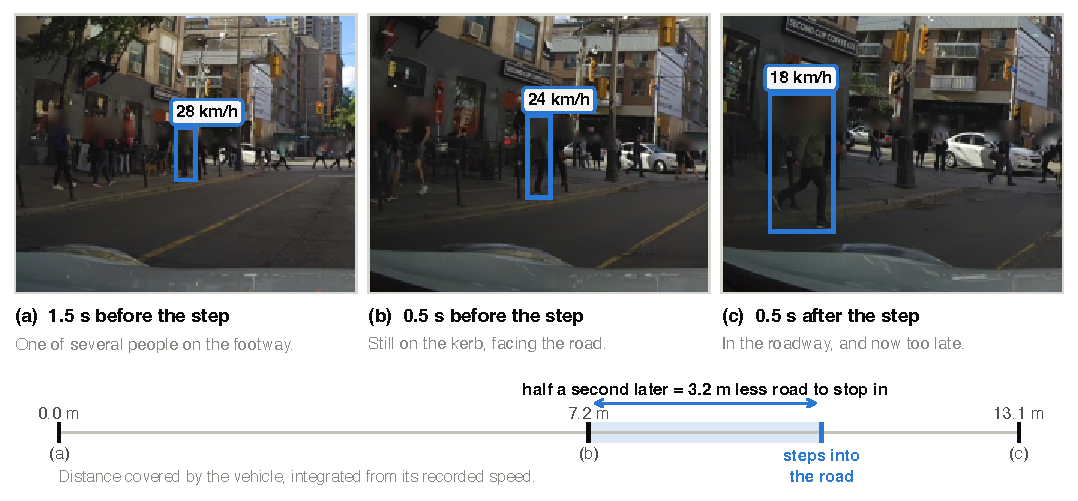
\includegraphics[width=\textwidth]{figures/fig_scenario.pdf}
\caption{The last two seconds before a crossing (PIE video 0016, pedestrian 3\_16\_919); boxes and speeds are the dataset's own. (\textbf{a}) 1.5\,s before the step, the subject is indistinguishable from the people who stay put; (\textbf{b}) 0.5\,s before; (\textbf{c}) 0.5\,s after, by which point the vehicle has travelled 13.1\,m. Head regions were irreversibly blurred before publication.\label{fig:scenario}}
\end{figure}

Figure~\ref{fig:stats} puts numbers on that scene. Road traffic crashes caused approximately 1.16 million deaths worldwide in 2025 and remained the leading cause of death among people aged 5--29~\citep{who2026factsheet,who2026roaddeaths}. Although the global rate of road traffic fatalities has decreased by 21\% since 2011, pedestrians still account for 23\% of the toll, second only to occupants of four-wheeled vehicles~\citep{who2023roadsafety}. The data from United States show it more closely. Pedestrian deaths reached a peak of 7,593 in 2022 before declining to 7,080 in 2024~\citep{nhtsa2026pedestrians}. The direction is right, but the level is not: the 2024 figure is still 29\% above the 5,494 of 2015, and in that decade pedestrians rose from 15\% to 18\% of all traffic deaths. State-reported data project a further 7\% decline for 2025~\citep{ghsa2026pedestrian}. The circumstances match the scene above rather than a marked crossing: of the 2024 deaths, 84\% were in urban areas, 73\% away from intersections and 76\% in the dark~\citep{nhtsa2026pedestrians}. These patterns highlight the importance of anticipating pedestrian crossing behavior before the pedestrian enters the roadway, particularly in complex urban and low-visibility environments where conventional signals or clearly defined crossing locations may not be available.

\begin{figure}[htbp]

\includegraphics[width=0.85\textwidth]{figures/fig1_pedestrian_statistics.pdf}
\caption{Pedestrians carry a disproportionate share of road traffic casualties, and one that has come down more slowly than the total. (\textbf{a}) Global road traffic deaths by road user type for 2021, the most recent breakdown published by the World Health Organization~\citep{who2023roadsafety}. (\textbf{b}) Pedestrians killed in the United States, 2015--2024~\citep{nhtsa2026pedestrians}.\label{fig:stats}}
\end{figure}

The focus of this study is anticipating whether a pedestrian is about to cross in such conditions. It differs from trajectory forecasting, which predicts an agent's future position or path and is scored by displacement-based metrics. Although the two tasks are related, they address different prediction objectives and should not be treated as interchangeable~\citep{rasouli2024diving}. The PIE dataset~\citep{rasouli2019pie} serves as a standard testbed because it provides over six hours of on-board video, per-frame pedestrian bounding boxes, synchronised vehicle telemetry, and annotated crossing events that define the prediction horizon. The benchmark introduced by Kotseruba et al.~\citep{kotseruba2021benchmark} standardised the observation window, prediction horizon, and recording-level data split, and most subsequent studies report results using this protocol, with models incorporating three to seven input streams and additional cues such as pose, optical flow, segmentation, or depth~\citep{azarmi2025pipnet,zhou2023pit}.

Despite the maturity of this benchmark, three methodological weaknesses recur. The first is that temporal leakage is rarely checked. Many PIE protocols anchor the observation window at the last annotated frame minus a fixed time-to-event offset. Nothing in that rule guarantees the window ends before the pedestrian steps into the road. When it does not, the task collapses from predicting an intention into detecting an event already in progress. The dataset authors note a related misalignment between how intention and action samples are anchored~\citep{rasouli2024diving}, but we know of no study that measures how often it happens. The second is that recent models are heavy. Three to seven input streams need pose estimators, optical-flow networks, segmentation or depth models to supply them at inference time. Each of those is another model to run, and the cost sits awkwardly on embedded automotive hardware~\citep{azarmi2025pipnet,xie2025gtranspdm}. The third is that evaluation is often thin. Results rest on a single split and on single-seed ablations. Point estimates arrive without intervals. Ground-truth boxes stand in for a real detector. Hyperparameters go unjustified~\citep{rasouli2024diving,azarmi2024featureimportance}.

One thing this paper does not claim is that minimal inputs are a new idea. Prediction from bounding boxes and ego-vehicle speed alone has been reported before~\citep{chen2024pedcmt,achaji2022attention}, and the pose-free ablation of GTransPDM~\citep{xie2025gtranspdm} demonstrates it inside a single paper. Section~\ref{sec:related-work} sets out that precedent. What this paper adds is a protocol in which no model observes the crossing it is asked to predict, interval estimates in place of point estimates, and a controlled test of whether the encoder matters at all.

Our contributions are as follows:
\begin{itemize}
\item A quantified temporal-leakage audit of the common PIE protocol and a leakage-free re-extraction anchored at PIE's own crossing point, verified at 0\% window leakage (Sections~\ref{sec:leakage-protocol} and~\ref{sec:leakage-results}).
\item A re-evaluation of a parsimonious two-stream (bounding box $+$ ego-speed) model: bootstrap and pedestrian-cluster intervals, leave-one-set-out cross-validation, multi-seed ablations, a documented hyperparameter search, and a detector-in-the-loop test (Section~\ref{sec:results}).
\item A four-family architecture study. An LSTM, a Transformer, a GRU, and an un-gated RNN, trained under one identical engine and compared both at a matched configuration and at equal search budgets, prove statistically indistinguishable on the primary metric, so the input signal, not the architecture or its gating, decides (Section~\ref{sec:architecture}).
\end{itemize}

The primary metric named in the third contribution is F1. We report F1 first, then accuracy, then ROC-AUC and PR-AUC, F1 being the operating-point metric appropriate to an imbalanced decision in which a missed crossing costs more than a false alarm.

\section{Related Work}
\label{sec:related-work}

Pedestrian behaviour prediction spans several related tasks in autonomous driving, including crossing-intention prediction, action recognition, trajectory forecasting and collision-risk assessment~\citep{sharma2022survey,rasouli2024diving}. This paper addresses the first of these, and the work bearing on it has grown in two directions at once: the models have taken on more input modalities, while the protocol that scores them has stayed largely unexamined. In this section, we review prior work from four perspectives: benchmark datasets and evaluation protocols, predictive models and input modalities, evaluation methodology, and pedestrian--vehicle interaction.

\subsection{The PIE Benchmark and Its Protocol}

Pedestrian crossing-intention prediction has been shaped primarily by two datasets, JAAD and PIE. JAAD introduced an annotated corpus of pedestrian behaviour recorded from a moving vehicle, providing an early foundation for studying crossing-related behaviour~\citep{rasouli2017jaad}. However, it does not provide synchronised ego-vehicle telemetry or a clearly labelled crossing event, limiting its suitability for evaluating when a pedestrian is expected to cross~\citep{rasouli2017jaad,rasouli2024diving}. The PIE dataset addressed these limitations by combining on-board video with frame-level pedestrian bounding boxes, behavioural annotations, synchronised ego-vehicle information, and labelled crossing events~\citep{rasouli2019pie}. Its richer temporal and vehicle-context information has made PIE a widely used benchmark for pedestrian crossing-intention prediction~\citep{sharma2022survey}.

Kotseruba et al.~\citep{kotseruba2021benchmark} subsequently established a standardised evaluation protocol based on PIE, including a sixteen-frame observation window, a one-to-two-second prediction horizon, and a recording-level data split. Most subsequent studies have adopted this protocol, providing a common basis for model comparison~\citep{xie2025gtranspdm,azarmi2025pipnet,li2025mft}. However, the temporal placement of the observation window introduces an important methodological concern~\citep{kaufman2012leakage}. Windows are typically anchored to the end of the annotated pedestrian track rather than the crossing onset~\citep{kotseruba2021benchmark}. As noted by Rasouli and Kotseruba~\citep{rasouli2024diving}, this can misalign intention and action prediction, while aggregate metrics may obscure differences across prediction horizons. Cross-dataset studies also show that models performing well on one dataset may generalise poorly to another~\citep{gesnouin2022assessing,bokkasam2025iddped}. Yet, to our knowledge, prior work has not quantified how often standard PIE observation windows overlap the crossing event. We address this gap by auditing each window's temporal relationship to the labelled crossing onset and re-anchoring windows so that intention is evaluated strictly before crossing begins (Section~\ref{sec:leakage-protocol}).

\subsection{Multimodal Models and the Minimal-Input Counter-Current}

The models built on that benchmark have grown steadily wider. PCPA~\citep{kotseruba2021benchmark} combines a pedestrian crop, pose keypoints, the box trajectory and vehicle speed. Pedestrian Graph$+$~\citep{cadena2022pedgraph} adds a pose graph, and IntFormer~\citep{lorenzo2021intformer}, PIT~\citep{zhou2023pit}, BiPed~\citep{rasouli2021biped} and PedFormer~\citep{rasouli2023pedformer} bring attention and joint trajectory-action learning to the same inputs. PIP-Net~\citep{azarmi2025pipnet} and MFT~\citep{li2025mft} reach seven streams and four. Their shared limitation is the pipeline this implies. Every additional stream is a pose estimator, an optical-flow network or a depth model that must run before the predictor does, and none of these studies reports what the extra streams buy.

A counter-current asks whether they are needed at all. PedCMT~\citep{chen2024pedcmt} predicts crossing intention from bounding boxes and ego-vehicle speed alone and reports parity with heavier methods, the pose-free ablation of GTransPDM~\citep{xie2025gtranspdm} reaches the same conclusion by removing its own skeleton encoder, and Achaji et al.~\citep{achaji2022attention} asked whether attention over boxes is all that is required. Others restrict the input further, to boxes and ego velocity by design~\citep{liu2025occlusion} or to a single cropped frame~\citep{qu2025efficientpie}. These works establish that a minimal input suffices. None establishes why, and all were measured under the protocol whose leakage Section~\ref{sec:leakage-protocol} quantifies. We isolate each stream's contribution on leakage-free data. This is the second gap.

One assumption is shared across both camps. Nearly all of this work evaluates on annotated bounding boxes, which a deployed system does not have. Our pipeline supplies boxes from a detector and identities from ByteTrack~\citep{zhang2022bytetrack}, so we can report what the same model scores when its inputs are estimated. IDD-PeD~\citep{bokkasam2025iddped} stresses the same assumption from the data side.

\subsection{Evaluation and Model Comparison Practice}
\label{sec:eval-practice}

How a benchmark is scored decides what counts as progress on it. Two choices matter for an imbalanced binary decision. Accuracy is a poor summary when the classes are skewed, and precision-recall analysis is more informative than ROC analysis in that regime~\citep{davis2006precision,saito2015precision}. Any threshold or configuration chosen on the data used to report a result also biases that result~\citep{cawley2010overfitting}.

How a difference is tested matters as much. A single score from a single run cannot separate a real margin from run-to-run variation, and the recommended practice is to report distributions rather than point estimates~\citep{reimers2017reporting}. Bouthillier et al.~\citep{bouthillier2021variance} quantify that variation across sources of randomness and show it is often large enough to reverse a published conclusion. Where evaluation units are not independent, as overlapping windows from one pedestrian are not, resampling has to respect the clustering~\citep{fieldwelsh2007}, and contrasts between two systems are best computed on identical resamples~\citep{koehn2004significance}.

The same lesson has been learned repeatedly about architectures. Melis et al.~\citep{melis2018sota} re-evaluated language-model architectures under equal tuning and found a properly regularised LSTM beating the newer models it had supposedly lost to. The finding generalises. Most generative adversarial networks reach similar scores given enough hyperparameter optimisation~\citep{lucic2018gans}, and none of eight LSTM variants tuned across 5,400 runs beat the standard cell~\citep{greff2017odyssey}. Chung et al.~\citep{chung2014gru} compared gated cells at matched parameter counts. No comparable study exists for crossing-intention prediction, where an encoder is usually adopted rather than tested.

\subsection{Pedestrian--Vehicle Interaction}

Crossing is an interaction, not a solitary act. Work on pedestrian--vehicle communication has largely studied the explicit channel, asking what an automated vehicle should display so that a pedestrian understands its intent~\citep{rouchitsas2019ehmi,alhawiti2024ehmi}. Its limitation for our purposes is that the channel is studied in one direction only. Our ego-speed result points the other way, since the vehicle's own motion, which pedestrians are known to read, is also the most informative input to a model predicting the pedestrian.

That result is confirmatory rather than new. A contextual feature-importance analysis reaches the same conclusion about ego speed and warns that relying on it may introduce a driver-side bias in yielding scenarios~\citep{azarmi2024featureimportance}. We adopt the finding and the caveat together, and Section~\ref{sec:discussion} states how far the caveat bounds our conclusions.

A fourth gap joins the three named in Section~\ref{sec:introduction}. Temporal encoders are adopted rather than compared at equal search budgets, so the architecture behind a published number is rarely the one that was tested. Sections~\ref{sec:methods} through~\ref{sec:results} address all four in that order.

\section{Materials and Methods}
\label{sec:methods}

Only one thing changes at a time. Every model reported here sees the same data, splits, loss, optimiser and stopping rule, is scored by the same code, and trains through one model-agnostic engine. Only the temporal encoder differs across families, and in each ablation only the ablated factor. A difference between two rows of a results table is therefore architectural, not an artefact of implementation or hardware.

\subsection{The PIE Dataset and Splits}

The Pedestrian Intention Estimation (PIE) dataset~\citep{rasouli2019pie} provides over six hours of driving recorded in downtown Toronto at $1920 \times 1080$ and 30 fps across six recording sets. Each pedestrian carries per-frame bounding boxes, a per-frame \texttt{cross} state, a binary crossing label and a \texttt{crossing\_point} event frame, with on-board diagnostics supplying synchronised vehicle speed. Parsing yields 582,376 frame-level rows covering 1,374 pedestrians once those labelled \texttt{crossing\_label}~$=-1$ are dropped.

We split by recording set rather than at random: set01, set02 and set04 train, set05 and set06 validate, set03 tests. Recording sets partition the videos, so no pedestrian, scene or video appears in more than one split, which a random split over windows would not guarantee. Two conventions circulate under the name of the standard protocol, the benchmark of Kotseruba et al.~\citep{kotseruba2021benchmark} training on set01, set02 and set06 while the dataset's toolkit defaults to the assignment we use; set03 tests under both, so published numbers stay broadly commensurable.

The training split holds 1,366 negative and 812 positive windows, a ratio of 1.682. That ratio is the positive-class weight in the training loss, computed after the split; over the pooled data it would have been 1.977, a value that would have seen the evaluation class distributions. Weighting is not the only option. Buda et al.~\citep{buda2018systematic} found oversampling dominant, but at ratios far more severe than this, so we swept the weight over $\{1.0, 1.3, 1.682, 2.1, 2.5\}$ on validation data and confirmed the anchor value.

\subsection{Temporal Leakage and the Leakage-Free Protocol}
\label{sec:leakage-protocol}

A model asked to predict whether a pedestrian will cross must not be shown the crossing. The widely used extraction anchors each window at the last annotated frame minus a time-to-event offset, which constrains nothing about where the crossing onset falls. Section~\ref{sec:related-work} sets out why that is a leakage risk and why no published study has measured it. PIE annotates a per-frame \texttt{cross} state the common parser discards, and recovering it turns the question into a count, reported in Section~\ref{sec:leakage-results}.

The fix uses an event the dataset already provides. We anchor at \texttt{crossing\_point}, truncate the contiguous track segment containing it at that frame inclusive, and slide 16-frame windows at 50\% overlap, keeping only those whose last observed frame falls 30 to 60 frames before the event. Pedestrians whose truncated track is shorter than the window plus the minimum look-ahead are excluded, costing 107 of 1,374 pedestrians (7.8\%). Figure~\ref{fig:protocol} contrasts the two rules.

\begin{figure}[htbp]
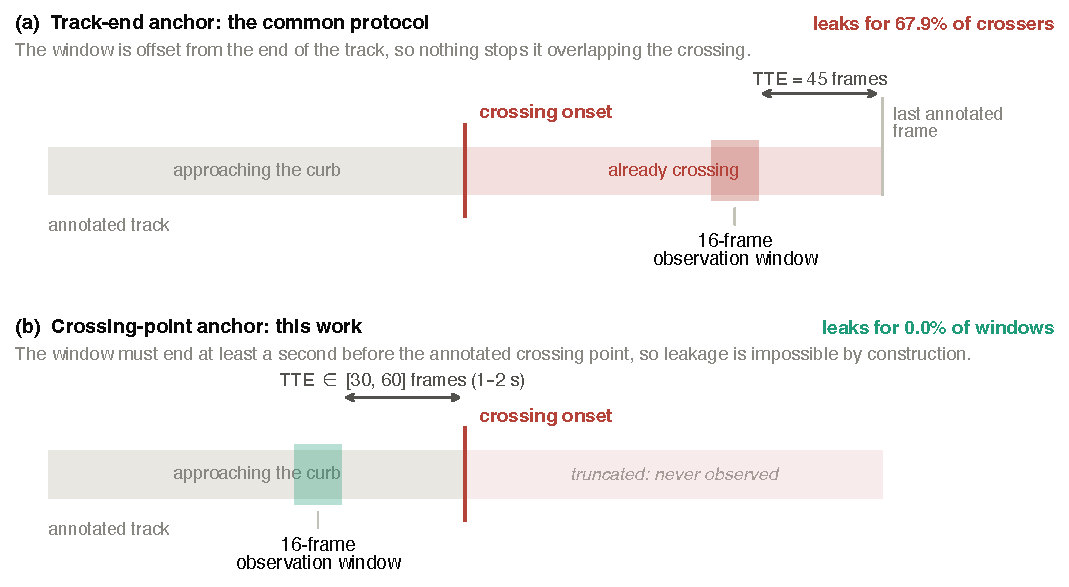
\includegraphics[width=0.8\textwidth]{figures/fig3_protocol.pdf}
\caption{Where the sixteen-frame observation window falls under each anchoring rule on PIE. (\textbf{a}) A track-end anchor places no constraint on the crossing onset, so the window may overlap the crossing it is meant to predict; this occurs for 67.9\% of crossing sequences. (\textbf{b}) Anchoring at \texttt{crossing\_point} with a 30--60 frame look-ahead makes that overlap impossible, verified at 0 of 4,906 windows.\label{fig:protocol}}
\end{figure}

Two properties make the result leak-free by construction rather than by inspection. First, \texttt{crossing\_point} coincides with the first frame labelled as crossing for 516 of 519 crossers (99.4\%) and never precedes it, so truncating there cannot leave crossing frames behind; second, the 30-frame minimum look-ahead separates the last observed frame from the event by at least one second. Re-running the audit confirms it: 0 of 4,906 windows contain a crossing frame, and the median gap moves from $+182$ frames to $-44$. Two consequences follow. The re-extraction is 3.5 times larger, because sliding windows over truncated tracks recovers samples one-window-per-track discards, and the best validation checkpoint moves from epoch 3 to epoch 17, the signature of a harder problem. Table~\ref{tab:protocol} reports both protocols side by side.

\begin{table}[htbp]
\caption{Track-end versus \texttt{crossing\_point} anchoring on PIE. Re-anchoring removes all window leakage and grows the usable sample 3.5-fold. Window counts are total (train/validation/test); the class weight is the positive-class weight in the training loss; rank-biserial correlations measure how well the bounding box at the last observed frame alone separates crossers from non-crossers.\label{tab:protocol}}
\begin{tabularx}{\textwidth}{lCC}
\toprule
\textbf{Property} & \textbf{Track-end anchor} & \textbf{\texttt{crossing\_point} anchor}\\
\midrule
Anchor rule & last annotated frame $-$ TTE & \texttt{crossing\_point}, TTE $\in [30,60]$\\
Sampling & one window per segment & 50\% overlap, stride 8\\
Windows (train/val/test) & 1389 (616/186/587) & 4906 (2178/634/2094)\\
Positive rate & 41.0\% & 33.6\%\\
Crossers observed mid-crossing & 387/570 (67.9\%) & 0/1648 (0.0\%)\\
Windows containing a crossing frame & 387/1389 (27.9\%) & 0/4906 (0.000\%)\\
Box area / height / bottom edge, rank-biserial & $+0.65 / +0.63 / +0.49$ & $+0.25 / +0.21 / +0.09$\\
Training class weight & 1.44 & 1.682\\
Best validation epoch & 3 & 17\\
\bottomrule
\end{tabularx}
\end{table}

\subsection{Features and Preprocessing}

Each window is sixteen frames, 0.53 s at 30 fps, of a five-dimensional vector: the four box coordinates and the ego-vehicle speed. Coordinates stay in raw pixels rather than being divided by the image dimensions, since a per-feature $z$-score removes any fixed scale factor and raw pixels keep the inference contract identical to the annotation format. The standardisation statistics come from the training split alone, because fitting any preprocessing step on evaluation data is itself leakage~\citep{kaufman2012leakage}. Unless a validation-tuned threshold is stated, decisions use 0.5 on the sigmoid output.

\subsection{Model Architectures}

All four families share one wrapper: a linear projection of the five inputs to 64 dimensions with a ReLU, a temporal encoder, a read-out from the pooled or final step, and a linear layer to a single logit. Only the encoder differs, so each comparison isolates one design choice, and every crossing-intention model here is trained from scratch; the only pretrained component is the detector in the live pipeline, which enters no tabulated comparison.

The bidirectional LSTM~\citep{hochreiter1997lstm,schuster1997bilstm} is the reference: two layers, hidden size 128, dropout 0.3, 594,561 parameters. Swapping \texttt{nn.LSTM} for \texttt{nn.GRU}~\citep{cho2014gru,chung2014gru} gives the gated recurrent twin at 446,081 parameters, isolating which gated cell is used; swapping it for a bidirectional tanh \texttt{nn.RNN}~\citep{elman1990rnn,rumelhart1986backprop} removes gating altogether at 149,121 parameters, isolating gating itself. The three form a ladder: if the LSTM's gates carry the task, removing them should cost something measurable. The fourth family is a pre-layer-norm Transformer encoder~\citep{vaswani2017attention,xiong2020prelayernorm}, searched to four heads, width 128, feed-forward width 512, four layers, last-token pooling and sinusoidal positional encoding at 794,241 parameters, with an un-searched control at 268,417; an ablation replaces the LSTM's final-step read-out with additive attention~\citep{bahdanau2015attention}, at 611,265. How capacity is equalised across cells is a decision in its own right, stated in Section~\ref{sec:settings}.

\subsection{Metric Hierarchy, Evaluation, and Statistical Procedure}

We report F1 first, then accuracy, then ROC-AUC and PR-AUC. Section~\ref{sec:eval-practice} gives the part of this ordering the literature supports. It does not establish F1 as primary, and we do not claim that it does. The ordering is a reporting choice appropriate to an imbalanced, safety-critical decision. Model selection touches validation data only, the decision threshold being fitted on the validation split, and set03 is scored once per experiment with every choice already fixed.

Two properties of the test set govern the statistics. Its 2,094 windows come from 541 pedestrian tracks at 50\% overlap, so windows are not independent. We therefore resample whole pedestrians and quote those intervals wherever a confidence interval appears. Contrasts use paired bootstraps on identical resamples, so an interval describes the difference rather than each model's separate variability. Both procedures follow the practice reviewed in Section~\ref{sec:eval-practice}, at 10,000 resamples throughout. Two statistics are never mixed in one sentence: the per-seed mean over five seeds, which is what other papers report, and the five-seed probability ensemble, which is one deployable predictor and scores slightly higher.

\subsection{Live Perception-to-Prediction Pipeline}

To measure the model where its inputs are estimated rather than annotated, we run it behind a detector and a tracker. Frames go to a YOLO26-M person detector (Ultralytics YOLO, \url{https://github.com/ultralytics/ultralytics}), detections to ByteTrack~\citep{zhang2022bytetrack} for identity association, and each track keeps a rolling 16-frame buffer of box coordinates and ego speed standardised with the training statistics, with absolute PIE frame numbers preserved so the speed lookup stays aligned.

\section{Experimental Settings}
\label{sec:settings}

Training, the statistical analysis, the recurrent searches and all timing ran on an Apple M4 with ten CPU cores and 16 GB of unified memory. The larger Transformer search and the observation-length sweeps used a Kaggle NVIDIA T4. Every configuration appearing in a table was then retrained locally through the same engine, with inference parity verified at about $10^{-6}$, so no tabled number depends on the machine that produced it. The stack is Python 3.13.5, PyTorch 2.12.0~\citep{paszke2019pytorch}, NumPy 2.4.6, SciPy 1.17.1 and scikit-learn 1.9.0, with Ultralytics 8.4.68 in the live pipeline.

One measured property of the hardware decides where recurrent runs execute. Training \texttt{nn.LSTM} on Apple's MPS backend is process-history-dependent: the same configuration and seed give different results according to what ran earlier in the same process. CPU training is bit-reproducible and context-free, and Transformer training does not show the effect, so recurrent runs needing exact reproduction execute on CPU, where the cross-family replication was done.

The training recipe is frozen and shared: binary cross-entropy with a positive-class weight of 1.682 in the training gradient only, Adam~\citep{kingma2015adam} with weight decay $10^{-5}$, batch size 32, at most 100 epochs, early stopping with patience 15, and a plateau scheduler halving the learning rate after five epochs without improvement. Each configuration is trained with five seeds, $[42, 0, 1, 2, 3]$, keeping the best validation epoch under whichever rule is in force and never the last, and set03 is evaluated once per experiment on that checkpoint. One configuration departs from the shared recipe: the tuned Transformer's F1 arm uses a positive-class weight of 2.5, chosen by its own validation sweep.

Search budgets were fixed in advance. The three recurrent families received an identical grid over learning rate $\{10^{-3}, 5\times10^{-4}, 10^{-4}\}$, dropout $\{0.2, 0.3, 0.5\}$, hidden size $\{64, 128, 256\}$ and depth $\{1, 2\}$, 54 nominal cells collapsing to 36 since inter-layer dropout is inert at depth 1, selected in three stages: all 36 at one seed, then the top five and the hand-set baseline across five seeds, and only then the winner and baseline on test. The single-seed leader was not the five-seed winner, which is what the second stage is for. The Transformer received 78 configurations, having more architectural freedom than a cell swap allows. No stage of any search evaluated the test set.

The comparison is then run twice, for the reason set out in Section~\ref{sec:eval-practice}: an architecture comparison measures tuning effort as much as architecture. In the tuned design each family selects its own configuration under an identical budget. The apparent alternative, one recipe for all four, sounds fairer and is not: it relocates the bias onto whichever family that recipe suits. Our own searches show it, the un-gated RNN selecting a learning rate an order of magnitude below the LSTM's; training it at the LSTM's rate would have measured how well an un-gated cell tolerates a rate chosen for a gated one.

The matched design answers the complementary question and carries a problem of its own. Holding the recurrent width at 128 keeps the cell swap as the only manipulation, but capacity does not follow width evenly: an LSTM carries four gate matrices where the un-gated cell carries one and the GRU three, giving 594,561, 149,121 and 446,081 parameters. Chung et al.~\citep{chung2014gru} handled this the other way, sizing each model to approximately equal parameter counts. We match width because a cell swap requires it, and report parameter counts in every table so either reading stays available. The asymmetry works against our own conclusion, since the gated cells hold a fourfold capacity advantage and any tie is reached by the smaller model. Five seeds is too small for a well-powered test across runs, so seed spread is descriptive and every comparative claim rests on the bootstraps of Section~\ref{sec:methods}, resampling 541 test pedestrians. Table~\ref{tab:hparams} gives what each search selected.

\begin{table}[htbp]
\caption{The configuration selected by each family's own search under the F1-first rule. Everything not listed is identical across families: batch size 32, at most 100 epochs, patience 15, train-only $z$-score standardisation, Adam with weight decay $10^{-5}$, and five seeds. Width is the recurrent hidden size, the read-out being twice this, or the Transformer's model and feed-forward dimensions; $\tau$ is tuned on validation data only.\label{tab:hparams}}
\begin{tabularx}{\textwidth}{lCCCCCCC}
\toprule
\textbf{Family} & \textbf{Width} & \textbf{Layers} & \textbf{Dropout} & \textbf{LR} & \textbf{Weight} & \textbf{$\tau$} & \textbf{Params}\\
\midrule
LSTM & 256 & 2 & 0.3 & $10^{-3}$ & 1.682 & 0.52 & 2,237,313\\
Transformer & 128/512 & 4 & 0.1 & $10^{-3}$ & 2.5 & 0.65 & 794,241\\
GRU & 256 & 2 & 0.3 & $5\times10^{-4}$ & 1.682 & 0.53 & 1,678,209\\
RNN & 256 & 2 & 0.2 & $10^{-4}$ & 1.682 & 0.53 & 560,001\\
\bottomrule
\end{tabularx}

\noindent{\footnotesize The Transformer uses four attention heads, last-token pooling and sinusoidal positional encoding; the recurrent families are bidirectional and read out from the final step.}
\end{table}

\section{Results}
\label{sec:results}

\subsection{The Temporal-Leakage Audit}
\label{sec:leakage-results}

Two thirds of the positive class is observed mid-crossing. Under the track-end anchor, 387 of 570 crossing sequences (67.9\%) contain at least one frame in which the pedestrian is already crossing, and 369 (64.7\%) are crossing throughout, leaving 183 with a clean window (Figure~\ref{fig:leakage}a). The median gap to crossing onset is $+182$ frames, almost six seconds into the event. A static shortcut is the second symptom: the box at the anchor frame separates the classes on its own, at rank-biserial $+0.65$ for area, $+0.63$ for height and $+0.49$ for the bottom edge (Figure~\ref{fig:leakage}b).

Re-anchoring at \texttt{crossing\_point} removes both. No window among the 4,906 contains a crossing frame, and the correlations fall to $+0.25$, $+0.21$ and $+0.09$. The shortcut collapsing alongside the leakage shows the two were connected: part of what made crossers look distinctive was that they were observed mid-crossing, close to the camera and low in the frame.

\begin{figure}[htbp]
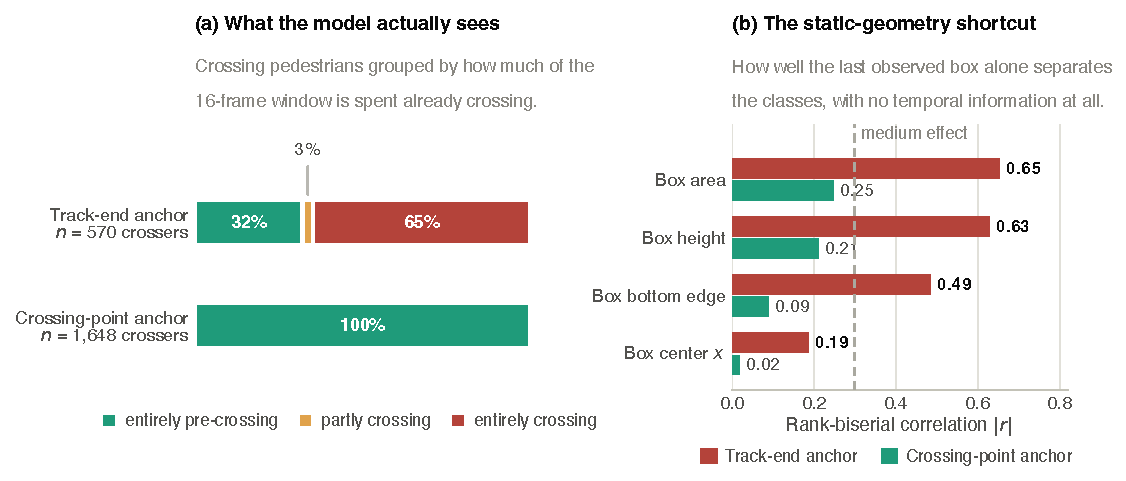
\includegraphics[width=0.85\textwidth]{figures/fig4_leakage.pdf}
\caption{The temporal-leakage audit on PIE, from the dataset's own per-frame \texttt{cross} annotations. (\textbf{a}) Crossing sequences grouped by how many of the sixteen observed frames already show crossing, under each anchoring rule. (\textbf{b}) How well the last observed box alone separates the classes, as rank-biserial correlation.\label{fig:leakage}}
\end{figure}

\subsection{Main Result}

On the leakage-free protocol the reference bidirectional LSTM reaches F1 $0.828 \pm 0.012$, accuracy $0.883 \pm 0.009$ and ROC-AUC $0.932 \pm 0.011$ over five seeds, with PR-AUC 0.876 against a base rate of 32.5\%. The bootstrap 95\% interval on AUC is $[0.92, 0.95]$ resampling windows and $[0.92, 0.96]$ resampling the 541 test pedestrians as clusters. The best F1 obtained by any model here is $0.852 \pm 0.012$, from the tuned un-gated RNN.

The AUC before the leakage was removed was 0.931. After removal it is 0.932. This near-identity is the finding, not a reassurance about it. A protocol showing two thirds of its positive windows mid-crossing produced the same headline number as one that shows none, so that number was never diagnostic of whether the task was prediction or detection.

The obvious alternative explanation is that the new protocol is simply easier, since it yields 3.5 times more data. Four checks rule that out. Scoring per window gives AUC 0.9131 and averaging within each pedestrian 0.9143, so the 50\% overlap inflates nothing. Restricting to tracks long enough for the stricter benchmark filter gives 0.9194, and the short tracks our looser floor admits score 0.8634 on their own. The additional windows are harder than the ones they join.

\subsection{Does the Architecture Matter?}
\label{sec:architecture}

Table~\ref{tab:families} reports all four families under both designs, with the two ablations. Under the tuned design the four F1 values span 0.844 to 0.852, a range of 0.008 against per-seed standard deviations of 0.008 to 0.017, and every cross-family contrast on F1 is a tie. Against the tuned LSTM, the GRU gives $\Delta$F1 $+0.0071$ with a 95\% pedestrian-cluster interval of $[-0.0043, +0.0187]$, the un-gated RNN $+0.0033$ $[-0.0083, +0.0150]$, and the Transformer $+0.0008$ $[-0.0124, +0.0142]$ at $p = 0.762$; the RNN against the GRU gives $-0.0038$ $[-0.0117, +0.0039]$. Every interval spans zero (Figure~\ref{fig:forest}a). We report these as ties and not as a win for the RNN, whose point estimate is nominally highest, because the intervals do not license an ordering.

A tie is only informative if the test can detect a difference, and on this data it can. The same paired bootstrap finds the F1-optimised LSTM better than its own AUC-selected baseline by $+0.0187$ $[+0.0073, +0.0300]$, surviving cluster resampling at $[+0.0043, +0.0349]$; the searched Transformer better than the AUC-selected LSTM on AUC by $+0.0135$ $[+0.0097, +0.0174]$; and the ego-speed ablation separated from everything by a margin no interval comes near.

On AUC the searched Transformer does have an advantage, $0.950 \pm 0.003$ against the LSTM's $0.932$, at a five-seed paired $t$-test of $p = 0.025$. The location of that advantage is the more useful result. Running the same Transformer architecture with the LSTM's own un-searched recipe gives $\Delta$AUC $+0.0005$ $[-0.0034, +0.0043]$, a tie: attention does not beat recurrence on this signal, and a search budget spent on architecture and recipe found a better configuration. The un-gated RNN closes the same gap given the same treatment, at $\Delta$AUC $-0.0013$ $[-0.0041, +0.0015]$ against the searched Transformer, while the GRU does not, at $-0.0070$ $[-0.0101, -0.0038]$.

\begin{table}[htbp]
\caption{All four families on the leakage-free PIE test set (set03, 2,094 windows, 32.5\% positive) under both comparison designs, with two ablations of the reference model. Values are per-seed means over five seeds. In the matched design the recurrent families share width 128 so that only the cell changes. ($\dagger$) Attention has no hidden-size equivalent, so the matched Transformer is the un-searched default, and is the one row selected on validation F1 rather than validation AUC. No cross-family difference in either design is significant on F1 (Figure~\ref{fig:forest}a).\label{tab:families}}
\begin{tabularx}{\textwidth}{llCCCC}
\toprule
\textbf{Design} & \textbf{Family} & \textbf{Params} & \textbf{F1} & \textbf{Acc} & \textbf{AUC}\\
\midrule
\multirow{4}{*}{Matched} & LSTM & 594,561 & 0.828 & 0.883 & 0.932\\
 & GRU & 446,081 & 0.840 & 0.898 & 0.933\\
 & RNN & 149,121 & 0.836 & 0.889 & 0.942\\
 & Transformer \textsuperscript{$\dagger$} & 268,417 & 0.821 & 0.878 & 0.942\\
\midrule
\multirow{4}{*}{Tuned} & LSTM & 2,237,313 & 0.844 & 0.897 & 0.940\\
 & Transformer & 794,241 & 0.847 & 0.896 & 0.947\\
 & GRU & 1,678,209 & 0.849 & 0.901 & 0.941\\
 & RNN & 560,001 & \textbf{0.852} & 0.902 & 0.948\\
\midrule
\multirow{2}{*}{Ablation} & LSTM, box only & 594,497 & 0.551 & 0.744 & 0.753\\
 & LSTM $+$ attention & 611,265 & 0.821 & 0.879 & 0.925\\
\bottomrule
\end{tabularx}
\end{table}

\begin{figure}[htbp]
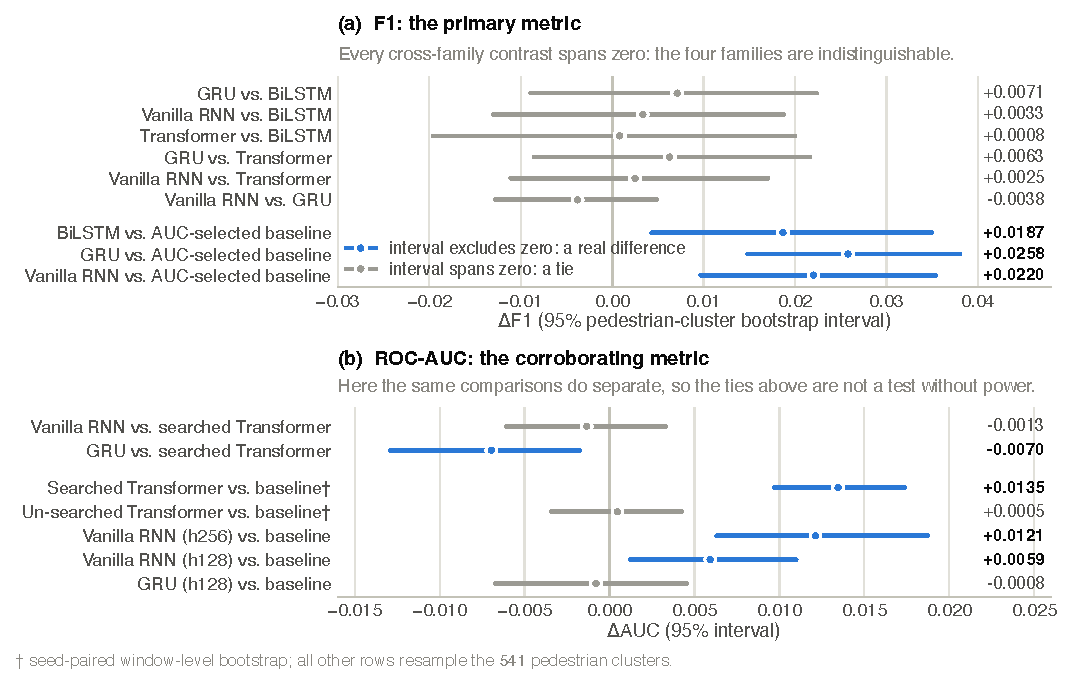
\includegraphics[width=0.82\textwidth]{figures/fig6_forest_compact.pdf}
\caption{Paired contrasts computed on identical resamples of the test set, with 95\% pedestrian-cluster bootstrap intervals over the 541 test pedestrians. (\textbf{a}) On F1, every cross-family contrast spans zero, while the lower group shows the same procedure detecting effects that are real. (\textbf{b}) On ROC-AUC the models do separate, with matched-configuration contrasts shown beside tuned ones.\label{fig:forest}}
\end{figure}

\subsection{Comparison with Published Baselines}

Table~\ref{tab:baselines} places our models against published PIE results. Two facts about it, stated rather than ranked. The highest F1 in the table is PIP-Net's 0.88, at a 0.5 s horizon with seven input streams. The highest among methods evaluated at a horizon comparable to ours is PedFormer's 0.87, with our four families 0.02 to 0.03 below it on two streams.

The horizon column exists because horizon dominates this comparison, and our own ablation is the evidence. On a fixed cohort of 493 test pedestrians, AUC falls from 0.961 at a 1.0 s horizon to 0.919 at 2.0 s (Section~\ref{sec:horizon}). Cross-paper differences of the size seen here are within the range horizon alone can produce.

Three further caveats belong with the table. Our protocol is leakage-free and the tabulated protocols are not, so the comparison is indicative and not a like-for-like leaderboard. The reference benchmark's code computes ROC-AUC on thresholded predictions instead of continuous scores, so not every tabulated AUC is the same statistic as ours. And PedCMT~\citep{chen2024pedcmt}, comparable on boxes and ego speed alone, is not tabulated at all: no open-access version of its results exists, and its released code uses a random 70/15/15 split rather than the benchmark partition, so its numbers are not protocol-comparable.

\begin{table}[htbp]
\caption{Crossing prediction on PIE. Baseline figures are as reported by the cited sources, verified against each method's own paper where an accessible version exists; entries marked ($\ddagger$) were available only through another paper's comparison table. Our rows are per-seed means over five seeds at threshold 0.5. Our protocol is leakage-free and therefore not strictly identical to the protocols behind the other rows, so this table is indicative rather than a like-for-like leaderboard. ``n.r.'' marks a horizon we could not verify from a primary source.\label{tab:baselines}}
\begin{adjustwidth}{-\extralength}{0cm}
\begin{tabularx}{\fulllength}{lcccclL}
\toprule
\textbf{Method} & \textbf{Acc} & \textbf{AUC} & \textbf{F1} & \textbf{Horizon} & \textbf{Streams} & \textbf{Modalities}\\
\midrule
PCPA~\citep{kotseruba2021benchmark} & 0.87 & 0.86 & 0.77 & 1--2 s & 4 & box, pose, context, speed\\
Pedestrian Graph$+$~\citep{cadena2022pedgraph} $^\ddagger$ & 0.89 & 0.90 & 0.81 & n.r. & 2--3 & pose graph, ego\\
IntFormer~\citep{lorenzo2021intformer} & 0.89 & 0.92 & 0.81 & 1--2 s & 4 & box, crops, pose, speed\\
PIT~\citep{zhou2023pit} $^\ddagger$ & 0.91 & 0.92 & 0.82 & 1--2 s & 5 & multimodal\\
BiPed~\citep{rasouli2021biped} & 0.91 & 0.90 & 0.85 & 1--2 s & 4 & multimodal multitask\\
PedFormer~\citep{rasouli2023pedformer} & 0.93 & 0.90 & 0.87 & 1--2 s & 4 & multimodal multitask\\
GTransPDM~\citep{xie2025gtranspdm} & 0.90 & 0.87 & 0.82 & 1--2 s & 3 & box, pose, ego\\
GTransPDM, no pose~\citep{xie2025gtranspdm} & 0.92 & 0.90 & 0.86 & 1--2 s & 2 & box, ego motion\\
MFT~\citep{li2025mft} & 0.90 & 0.94 & 0.83 & 1--2 s & 4 & numerical context\\
PIP-Net~\citep{azarmi2025pipnet} & 0.92 & 0.94 & 0.88 & 0.5 s & 7 & box, pose, RGB, flow, semantics, depth, speed\\
\midrule
LSTM (ours) & 0.897 & 0.940 & 0.844 & 1--2 s & 2 & box, ego speed\\
Transformer (ours) & 0.896 & 0.947 & 0.847 & 1--2 s & 2 & box, ego speed\\
GRU (ours) & 0.901 & 0.941 & 0.849 & 1--2 s & 2 & box, ego speed\\
RNN (ours) & 0.902 & 0.948 & 0.852 & 1--2 s & 2 & box, ego speed\\
\bottomrule
\end{tabularx}
\end{adjustwidth}
\end{table}

\subsection{Which Input Carries the Signal?}

Removing ego-vehicle speed from an otherwise identical LSTM collapses it: F1 falls from 0.828 to 0.551, accuracy from 0.883 to 0.744 and AUC from 0.932 to 0.753. The bootstrap intervals do not approach each other, the box-only model topping out near 0.78 where the two-stream model starts at 0.92. Losing one of two inputs costs 0.18 AUC, which identifies ego speed as the dominant stream. The finding is confirmatory: a contextual permutation analysis reached it independently, and warned that reliance on ego speed may introduce a driver-side bias in yielding scenarios~\citep{azarmi2024featureimportance}. Adding capacity to the temporal model does nothing comparable, additive attention over the recurrent states moving AUC from 0.932 to 0.925 and F1 from 0.828 to 0.821, both within seed noise.

\subsection{Prediction Horizon and Observation Length}
\label{sec:horizon}

Horizon matters and window length does not. On the matched cohort of 493 test pedestrians eligible at every horizon, AUC falls from $0.961$ at 1.0 s to $0.946$ at 1.5 s and $0.919$ at 2.0 s, with every pairwise paired $t$-test at $p \le 0.004$ and Kruskal--Wallis $p = 0.002$; restricting all three conditions to a common cohort changes the numbers by at most 0.002. This overturns a conclusion we previously drew ourselves. On the leaky protocol the model appeared insensitive to horizon, which we now read as a symptom and not a finding: a model detecting an in-progress crossing is indifferent to the nominal distance to an event it is already observing.

Observation length behaves the other way. At 8, 16 and 30 frames, AUC is $0.931$, $0.933$ and $0.937$; no pairwise test reaches significance, the smallest $p$ being 0.21, and the between-condition spread of 0.0058 is smaller than the within-condition seed standard deviation of 0.0073. Extending to 32 and 64 frames lowers F1 for all four families, on a sweep that is not a matched cohort, since a longer window needs a longer pre-crossing track and the usable test set shrinks from 2,094 windows to 1,009 and then 458. One result stands out: at 64 frames the un-gated RNN alone falls behind, losing 0.050 F1 against its own 16-frame result where the gated cells lose 0.026 to 0.028. Per-seed intervals still overlap, so this is directional, but it bounds the equivalence result. Gating is redundant over half a second and begins to matter by two.

\subsection{Cross-Set Generalization, Capacity, and Latency}

Leave-one-set-out over all six recording sets gives AUC $0.928 \pm 0.041$, or $0.915 \pm 0.029$ excluding the 47-window set05 fold, which is too small to interpret. The fold holding out set03, our fixed test set, scores 0.931, sitting at the fold mean and not above it, so set03 is not an unusually easy partition; the other families behave similarly, at 0.946 for the GRU, 0.939 for the Transformer and 0.937 for the RNN.

Capacity is not the binding constraint. Hidden sizes 64, 128 and 256 give AUC $0.927$, $0.933$ and $0.938$, with 256 against 128 not significant at $p = 0.338$ despite 3.8 times the parameters; depths 1, 2 and 3 give $0.930$, $0.932$ and $0.931$, far inside seed noise. The 36-configuration grid search beat the hand-set baseline on test by $+0.0006$ at $p = 0.914$, which is to say it confirmed it.

Latency does not discriminate between these models. All four run far inside a real-time budget on CPU at batch 1, at 0.316 ms per window for the RNN, 0.459 for the Transformer, 0.575 for the LSTM and 0.721 for the GRU, or 46 to 105 times inside the 33.3 ms of a 30 fps frame. In the full pipeline the detector accounts for 92.7\% of per-frame cost and the intention model 4.5\%.

\subsection{Detector-in-the-Loop and Qualitative Behaviour}

Replacing annotated boxes with detected ones costs little. Across 311 windows from 98 pedestrians in two test clips, at mean IoU 0.750 between detected and annotated boxes, per-window AUC falls from 0.962 to 0.953 and per-pedestrian AUC from 0.958 to 0.948, with the thresholded decision flipping in 10 of 311 windows (3\%). Two limits on that number. It is a lower bound on deployed degradation, because detections are matched to annotations by best overlap, which isolates box-quality noise and removes the association errors a deployed system would make. And the pipeline's weak points are in perception, not prediction: the detector covers 88\% of pedestrians, so roughly one in eight is never tracked well enough to predict for at all, and a single ByteTrack identity covers a mean of 39\% of a pedestrian's frames, with 59\% of windows carrying a competing identity. Deployment would need re-identification before a better intention model.

Figure~\ref{fig:qualitative} shows the pipeline on those clips, scored by the five-seed LSTM ensemble at its validation-tuned threshold of 0.516. One pedestrian is flagged at $p = 0.71$ about 1.5 s before stepping off the kerb; a worker standing at a kerb beside a crosswalk is correctly left at $p = 0.31$. Both panels illustrate behaviour rather than sample it, so the failure rates above are the representative numbers. Across all 439 windows in these clips the ensemble gives 134 true positives, 16 false positives, 19 false negatives and 270 true negatives, an accuracy of 0.920 and F1 of 0.884.

\begin{figure}[htbp]
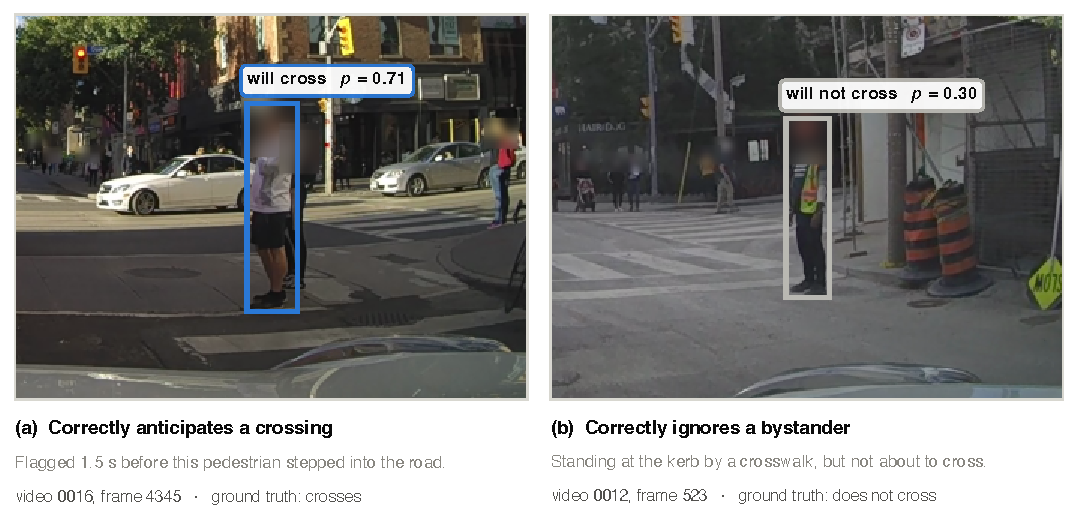
\includegraphics[width=\textwidth]{figures/fig9_qualitative.pdf}
\caption{The pipeline on two PIE test scenes, with boxes from YOLO26-M and ByteTrack rather than annotations, scored by the five-seed LSTM ensemble at threshold 0.516. (\textbf{a}) A pedestrian flagged at $p = 0.71$ about 1.5\,s before stepping into the road. (\textbf{b}) A worker at a kerb, correctly not flagged. Faces were irreversibly blurred before publication.\label{fig:qualitative}}
\end{figure}

\section{Discussion}
\label{sec:discussion}

Two cheap inputs get close to what heavier pipelines achieve. We are not the first to find it. PedCMT~\citep{chen2024pedcmt}, the pose-free ablation of GTransPDM~\citep{xie2025gtranspdm} and Achaji et al.~\citep{achaji2022attention} reported versions of the result before us, and EfficientPIE~\citep{qu2025efficientpie} has since pushed the input down to a single frame. What we add is that it survives a protocol in which no model ever observes the crossing it is asked to predict, that it holds under interval estimates over 541 resampled pedestrians, and that we can say where the predictive content sits. Removing ego speed collapses the model; replacing the temporal encoder three times moves F1 by less than the seed-to-seed spread. That places the information in the ego-speed profile and coarse box dynamics, both legible within half a second. For a practitioner the implication is about where effort belongs. On a fixed budget, improving the perception front end and the telemetry path will do more than replacing the sequence model, because our measurements put the binding constraints there, at 88\% detector recall and 39\% track-identity purity.

The second finding is about metrics, and it emerged from running the comparison two ways. On ROC-AUC the searched Transformer beats the LSTM by a margin whose interval excludes zero; on F1, after both families receive equivalent optimisation, they are indistinguishable. Neither is an error and neither is more valid: they answer different questions, one about ranking across all thresholds and one about a decision at an operating point, and which one a paper reports is a choice made before any model is trained. An architecture comparison fixing on one metric, one seed and unequal search budgets can produce a headline in either direction, and ours could have. Had we reported AUC from the searched Transformer against the LSTM's un-searched configuration we would have published a Transformer win; had we reported F1 at matched width without tuning, a null result about attention. The literature carries this warning already for language and generative models~\citep{melis2018sota,lucic2018gans}, and the defence is the same: tune every candidate under a stated budget, report more than one metric, and let intervals carry the comparison.

The leakage finding is the one most likely to matter outside this paper. It is a property of the protocol and not of our model, so any study anchoring windows at the end of an annotated track inherits it. Three symptoms let others recognise it without re-running our audit. Convergence is implausibly fast, since detecting an in-progress crossing is far easier than predicting one, our leaky runs peaking at epoch 3 against epoch 17 after the fix. Static geometry separates the classes on its own, because a pedestrian mid-crossing is close, large and low in the frame, so rank-biserial correlations above 0.6 for box area and height are a strong signal against the 0.25 and 0.21 that remain once the leakage is removed. And the clearest tell is insensitivity to the prediction horizon: a model that appears to predict two seconds ahead as well as one is probably not predicting at all, since genuine performance degrades with distance to the event, as ours does from 0.961 to 0.919. The audit is cheap, needing only the per-frame annotation the dataset already ships.

Several limitations bound these conclusions, and the largest is that all of them come from one dataset. PIE is a single city, vehicle and camera, and predictors robust within a dataset can degrade sharply across them~\citep{gesnouin2022assessing}, a pattern IDD-PeD reproduces with losses up to 15\%~\citep{bokkasam2025iddped}; replicating both audit and model elsewhere is ongoing work, and we report no cross-dataset number. Second, the instrumented vehicle was driven by a human who could see the pedestrian and slow in anticipation, so part of what the model reads is that driver's judgement rather than the pedestrian's behaviour; the field has flagged this and proposed proximity change rate as a partial substitute~\citep{azarmi2024featureimportance}, and a speed-perturbation study would quantify how much of our result depends on it. Third, our accuracy is mid-band, at 0.897 to 0.902 against PedFormer's 0.93, and we make no claim to be state of the art, only competitiveness at a fraction of the input cost. Fourth, our protocol is leakage-free and the tabulated ones are not, so Table~\ref{tab:baselines} is indicative and not a leaderboard, a caveat covering also the two split conventions in circulation and the AUCs computed on thresholded predictions. Fifth, the equivalence is bounded by horizon, since at 64 frames the un-gated RNN alone falls behind by 0.050 F1 against 0.026 to 0.028 for the gated cells, so gating is redundant over half a second but not indefinitely, and per-seed intervals still overlap. Sixth, the detector-in-the-loop result rests on two clips and 98 pedestrians with detections matched by best overlap, so its 0.009 AUC drop is a lower bound. Finally, five seeds is a small sample, and we have leaned on bootstraps over 2,094 windows and 541 pedestrians instead of tests across runs~\citep{bouthillier2021variance}.

\section{Conclusions}
\label{sec:conclusions}

The observation windows commonly used to evaluate crossing-intention prediction on PIE contain the event they are meant to precede. Measured against the dataset's own per-frame annotation, 67.9\% of crossing sequences are observed while the pedestrian is already in the road, and for most of those the crossing occupies the entire window, which makes the task detection, not prediction. Re-anchoring each window at the labelled crossing event and requiring a thirty-frame look-ahead removes this by construction, verified at zero of 4,906 windows, and yields 3.5 times as many usable windows.

On that protocol, a model given only a pedestrian bounding box and the ego-vehicle speed reaches F1 between 0.844 and 0.852 with ROC-AUC between 0.940 and 0.948, competitive with methods consuming three to seven streams. The input is what carries this. Removing ego speed drops F1 from 0.828 to 0.551, whereas exchanging the temporal encoder does not move the primary metric: the four families are statistically indistinguishable on F1, every cross-family interval spanning zero, and the un-gated cell ties the gated ones on a quarter of their parameters at matched width. The Transformer's ROC-AUC advantage is an artefact of search budget and not of attention, since the same architecture on an un-searched recipe ties the LSTM and an equally searched RNN closes the gap. The input signal, not the architecture, decides this task, and no comparison here rests on a point estimate.

Three directions follow. The audit and the model should both be replicated on a second dataset, the audit being cheap to run anywhere the annotation identifies a crossing onset. A speed-perturbation study would establish how much of the ego-speed result reflects the pedestrian's behaviour and how much a human driver anticipating them, the largest interpretive uncertainty we carry. And the perception front end deserves the attention the sequence model no longer needs: at 88\% detector recall and 39\% track-identity purity, it is detection and identity, not intention, that would limit a system of this kind in a vehicle.

\vspace{6pt}

%=================================================================
% Back matter, in the template's order
%=================================================================

\supplementary{The following supporting information can be downloaded at \linksupplementary{s1}, Video S1: 26 s of continuous output from the detection-to-prediction pipeline on a PIE test clip, with per-pedestrian crossing probabilities overlaid and all faces irreversibly blurred.}

\authorcontributions{Conceptualization, X.X. and Y.Y.; methodology, X.X.; software, X.X.; validation, X.X. and Y.Y.; formal analysis, X.X.; investigation, X.X.; data curation, X.X.; writing---original draft preparation, X.X.; writing---review and editing, X.X. and Y.Y.; visualization, X.X.; supervision, Y.Y.; project administration, Y.Y. All authors have read and agreed to the published version of the manuscript. PLACEHOLDER: initials to be completed by the authors.}

\funding{PLACEHOLDER: this research received no external funding.}

\institutionalreview{Not applicable. This study is a secondary analysis of the publicly available PIE dataset and involved no new experiments on humans or animals. Every face in the video frames reproduced in Figures~\ref{fig:scenario} and~\ref{fig:qualitative} and in Video S1 was irreversibly blurred before publication.}

\informedconsent{Not applicable.}

\dataavailability{The PIE dataset analysed in this study is publicly available from its authors at \url{https://data.nvision2.eecs.yorku.ca/PIE_dataset/}. The window-extraction code, the training engine, the trained model configurations and the analysis scripts that reproduce every number and figure in this paper are available at PLACEHOLDER: repository URL.}

\acknowledgments{During the preparation of this manuscript, the authors used Claude Code (Anthropic), Claude Opus, for drafting and editing text, for writing and debugging analysis and figure-generation code, for analysis and interpretation of results, and for literature search and verification. The authors have reviewed and edited the output and take full responsibility for the content of this publication.}

\conflictsofinterest{The authors declare no conflicts of interest.}

\abbreviations{Abbreviations}{%
The following abbreviations are used in this manuscript:\\

\noindent
\begin{tabular}{@{}ll}
ADAS & Advanced driver assistance system\\
AUC & Area under the receiver operating characteristic curve\\
CPU & Central processing unit\\
GRU & Gated recurrent unit\\
IoU & Intersection over union\\
LSTM & Long short-term memory\\
MPS & Metal Performance Shaders\\
OBD & On-board diagnostics\\
PIE & Pedestrian Intention Estimation dataset\\
PR-AUC & Area under the precision-recall curve\\
RNN & Recurrent neural network\\
ROC & Receiver operating characteristic\\
TTE & Time to event
\end{tabular}
}

%=================================================================
\begin{adjustwidth}{-\extralength}{0cm}

\reftitle{References}

\bibliography{references}

\PublishersNote{}
\end{adjustwidth}
\end{document}
